% !TEX root = main.tex
\chapter{Construction}

  This chapter concerns the construction of the rear wing. The step from theoretical abstraction to a real product. This includes dimensioning, material selection and finalizing the design. The simulated rear wing lacks a proper mounting method design, which is also included in this chapter.

\section{Requirements}

  The formula student competition has a clear ruleset dictating the dimensional requirements of aerodynamic devices. The most crucial elements are outlined below:

  \subsection{Dimensional Requirements}
    \begin{tcolorbox}
      Height Restrictions:
      \begin{itemize}
        \item[T7.3.1] All aerodynamic devices rearward of a vertical plane through the rearmost portion of the front face of the driver head restraint support, excluding any padding, set to its most rearward position must be lower than $\SI{1.2}{\metre}$ from the ground.
      \end{itemize}

      Width Restrictions:
      \begin{itemize}
       \item [T7.3.2] All aerodynamic devices higher than 500 mm from the ground, must not extend outboard of the most inboard point of the rear wheel/tire.
      \end{itemize}

      Length Restrictions:
      \begin{itemize}
        \item [T7.3.3] All aerodynamic devices must not extend further rearward than 250 mm from the rearmost part of the rear tires
      \end{itemize}

      Minimum Edge Radii of Aerodynamic Devices:
      \begin{itemize}
        \item[T7.4] All forward facing edges of aerodynamic devices that could contact a pedestrian must have a
      minimum radius of $\SI{5}{\milli\metre}$for all horizontal edges and 3 mm for vertical edges.
      \end{itemize}
    \end{tcolorbox}

    The dimensional requirements from the rules was sketched on the front plane of the car's CAD drawing. This allows positioning the wing in the square seen in figure \ref{fig:cadplacement}.

    \begin{figure}
      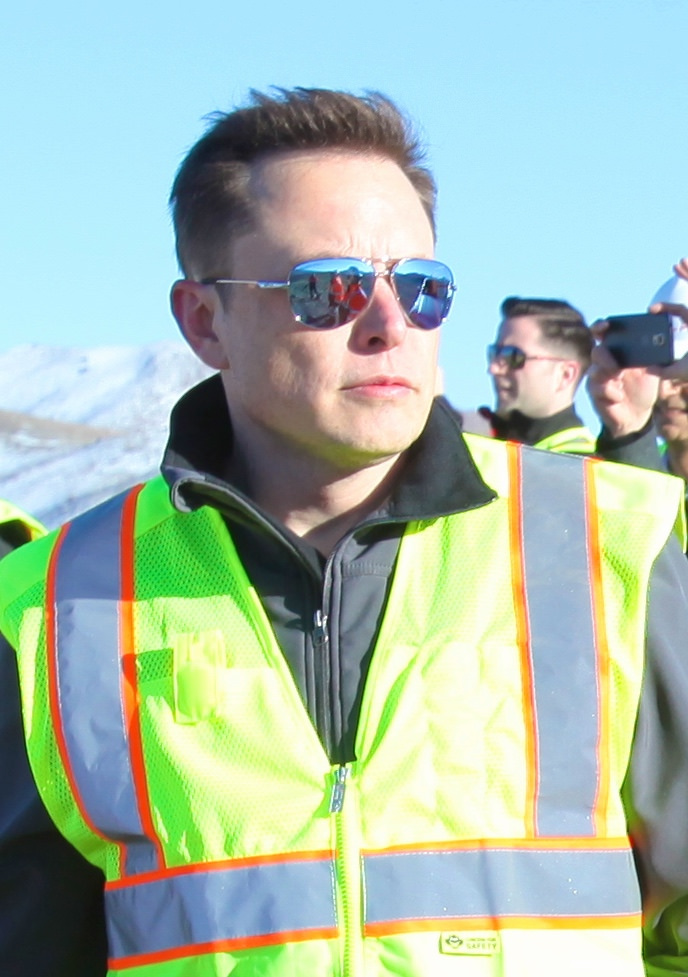
\includegraphics[width=.5\textwidth]{elon6}
      \caption{The ruleset above drawn against the design of the car. The marked square is the area where the wing can be freely placed.}
      \label{fig:cadplacement}
    \end{figure}

  \subsection{Strength Requirements}
    \begin{tcolorbox}
      Aerodynamic Devices Stability and Strength:
      \begin{itemize}
        \item [T7.5.1] Any aerodynamic device must be able to withstand a force of 200 N distributed over a minimum surface of $\SI{225}{\centi\metre\squared}$ and not deflect more than $\SI{10}{\milli\metre}$ in the load carrying direction.
        \item [T7.5.2] Any aerodynamic device must be able to withstand a force of $\SI{50}{\newton}$ applied in any direction at any point and not deflect more than $\SI{25}{\milli\metre}$.
      \end{itemize}
    \end{tcolorbox}

    As the wing will be mounted against the end plates, it can be considered a simply supported beam. The elastic deflection is thus described by:

    \begin{align}
      u &= \frac{FL^3}{48EI}
    \end{align}
    where $u$ is the deflection at the midpoint, $F$ is the force applied, $L$ is the length of the beam (the same as $b$ for wings), $E$ is the elastic modulus of the wing and $I$ is the moment of inertia of the cross section.

\section{Material Selection}\fxnote{Overvej CES (for flair jo)}

  Material selection was done based on the stress calcul

\section{Composites}
  \subsection{Sandwich Structure}
  \subsection{Wing Deflection}

\section{Final Design of Rear Wing}
  \fxnote{Presentation of CAD Drawings and method of how we will get to this result}
  \fxnote{Rendering}

  \subsection{Blue Prints}

\section{Manufacturing Final Design}
  \subsection{Polystyrene Molds}

  The molds for the wings were chosen as positive molds, meaning polystyrene molds of the actual wings were cut out and overlaid with resin coated carbon fiber. In order to do this, we devised a hotwire-based specialized tool for the job. This can be seen in figure \ref{fig:hotwire}, and the name of the job is to do it slowly in order to receive a clean surface.

  \begin{figure}
    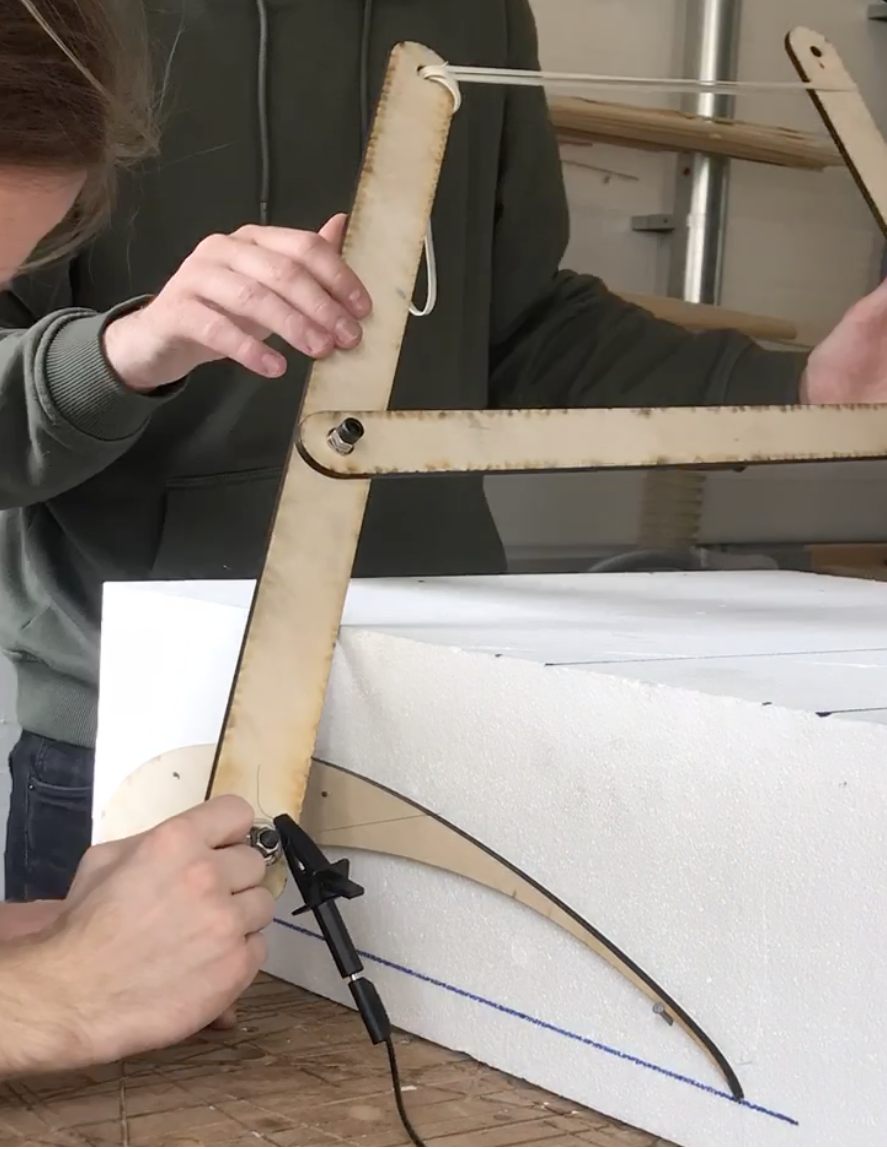
\includegraphics[width=\textwidth]{hotwiremethod}
    \caption{The hot wire melts the styrofoam while sliding along the wooden template.}
    \label{fig:hotwire}
  \end{figure}

  \subsection{Hand Layup}
    \begin{figure}
      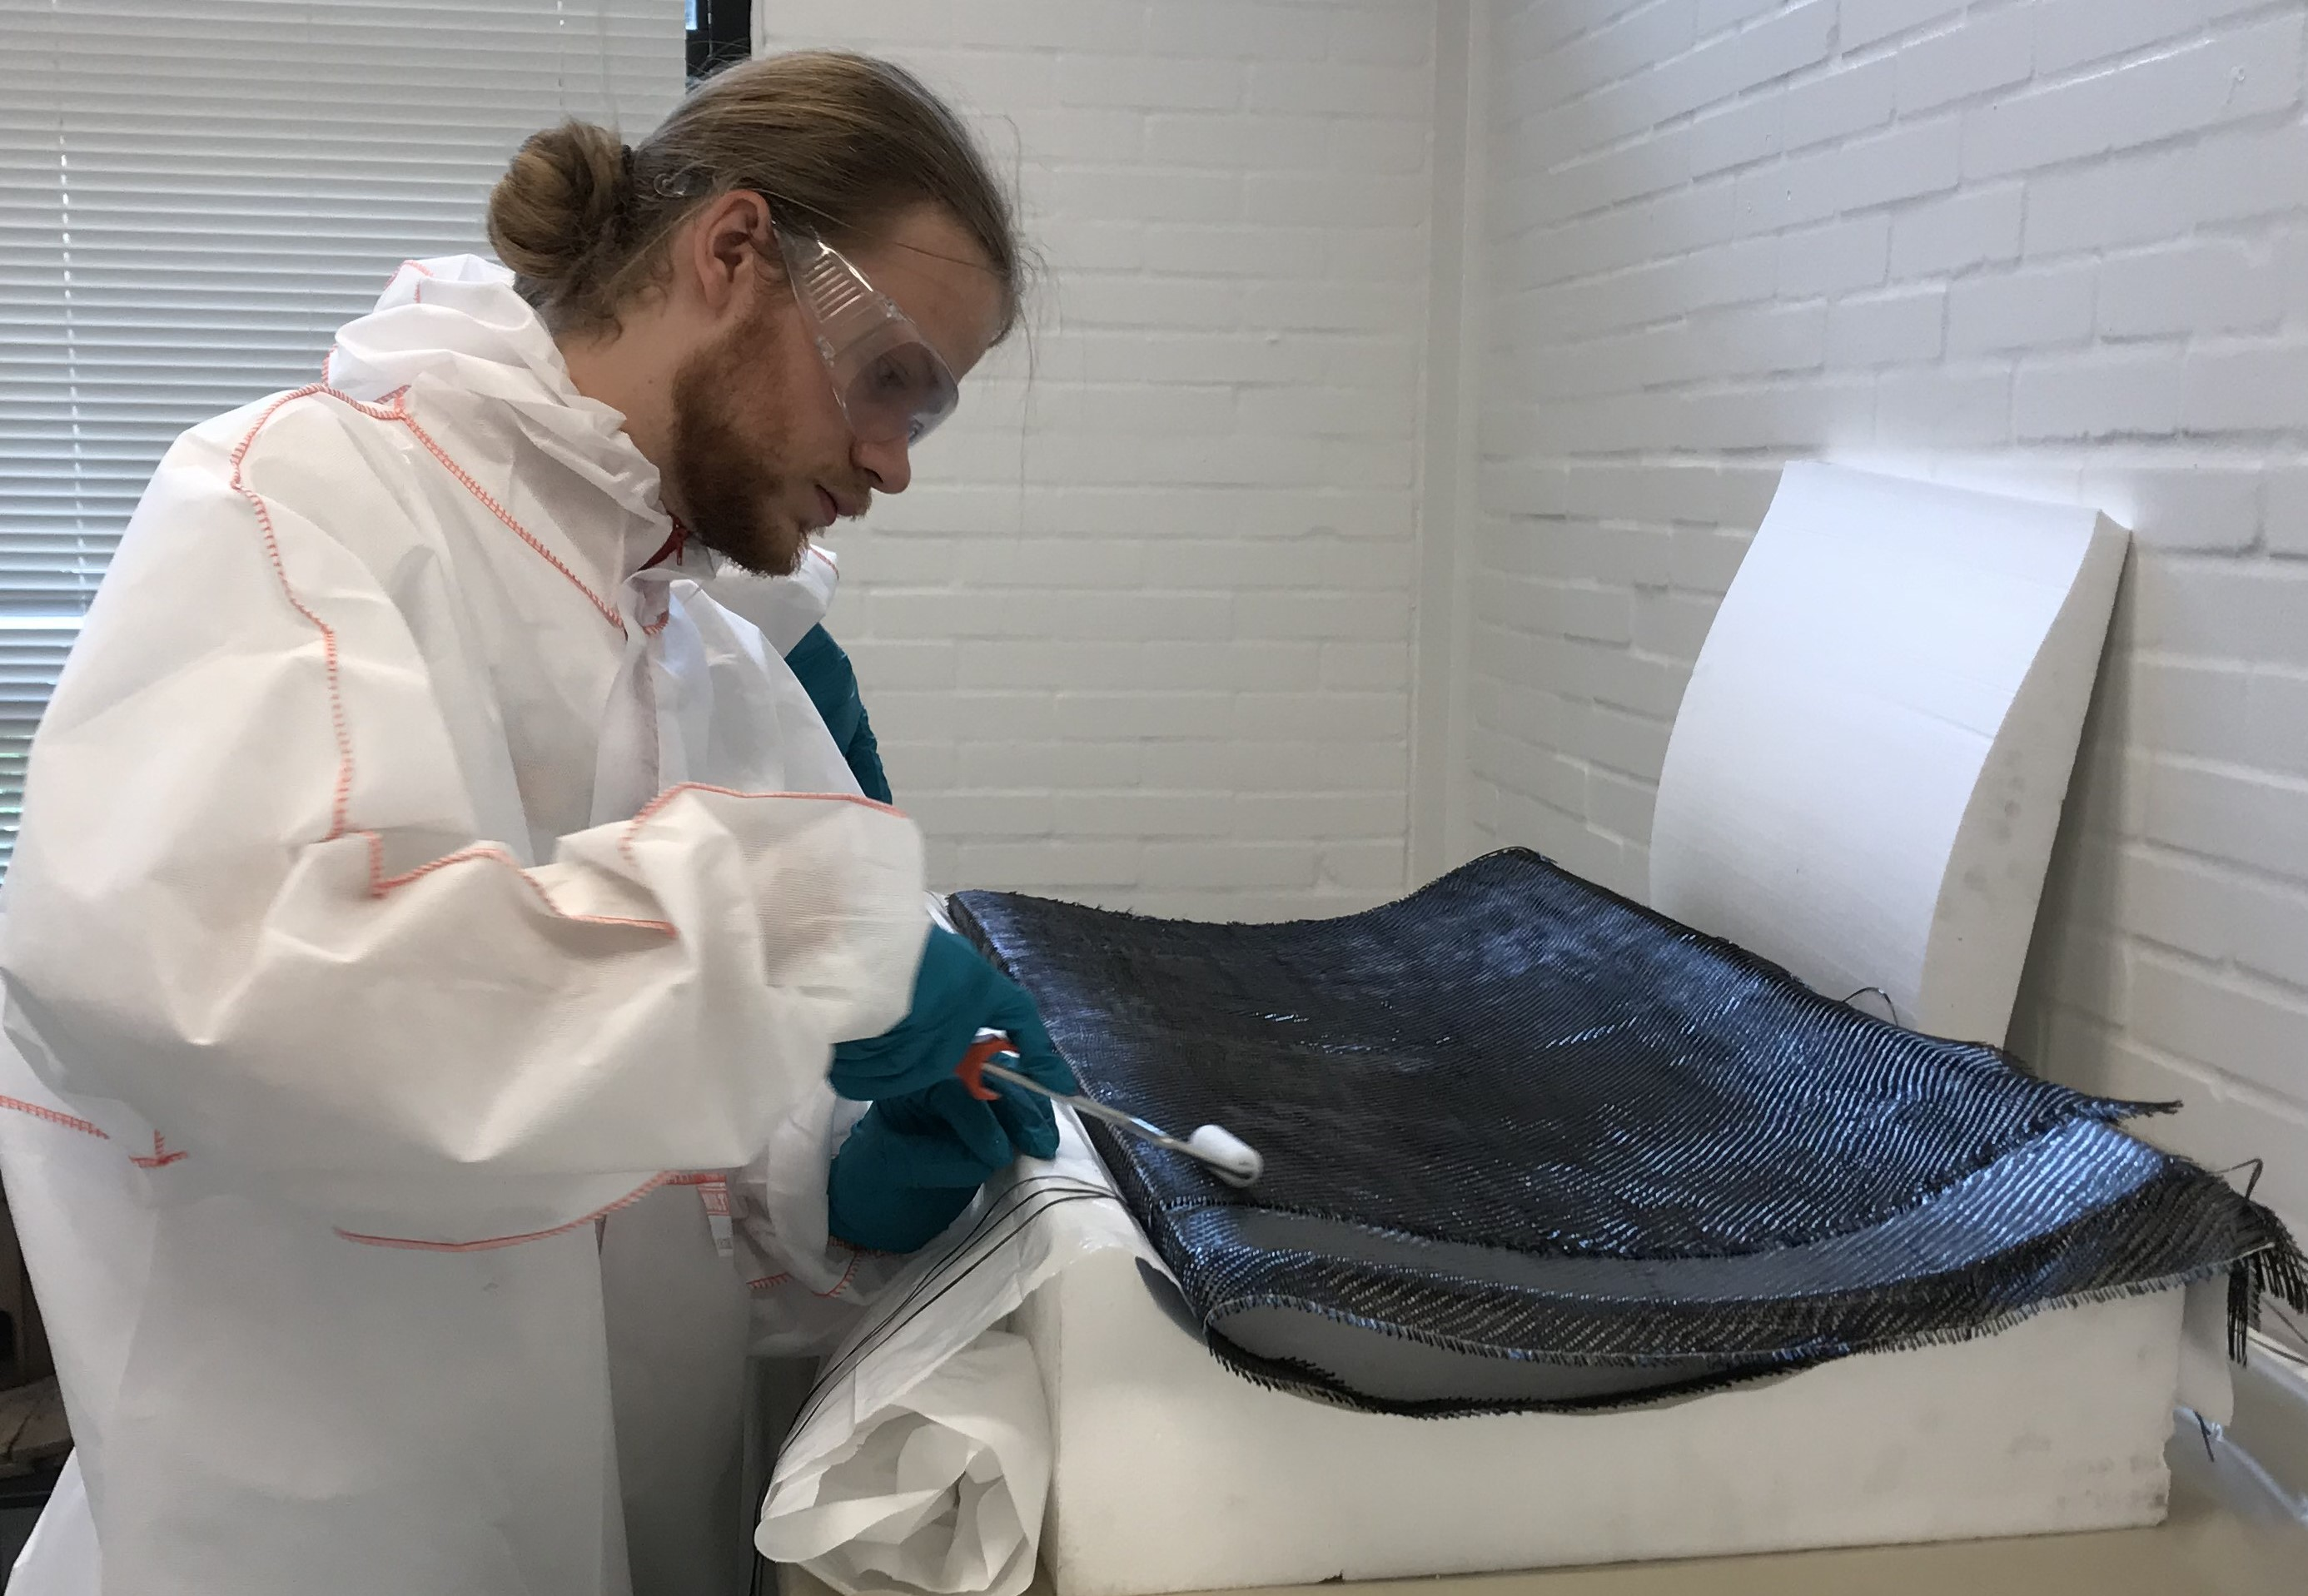
\includegraphics[width=\textwidth]{handlayupwnicolai}
      \caption{Steffan and Nicolai performing a hand layup of the carbon fiber mats around a polystyrene foam core.}
      \label{fig:handlayup}
    \end{figure}

    \fxnote{Show how we did the hand lay up. What went wrong what went well.}

  \subsection{Surface Finish}

    \begin{figure}
      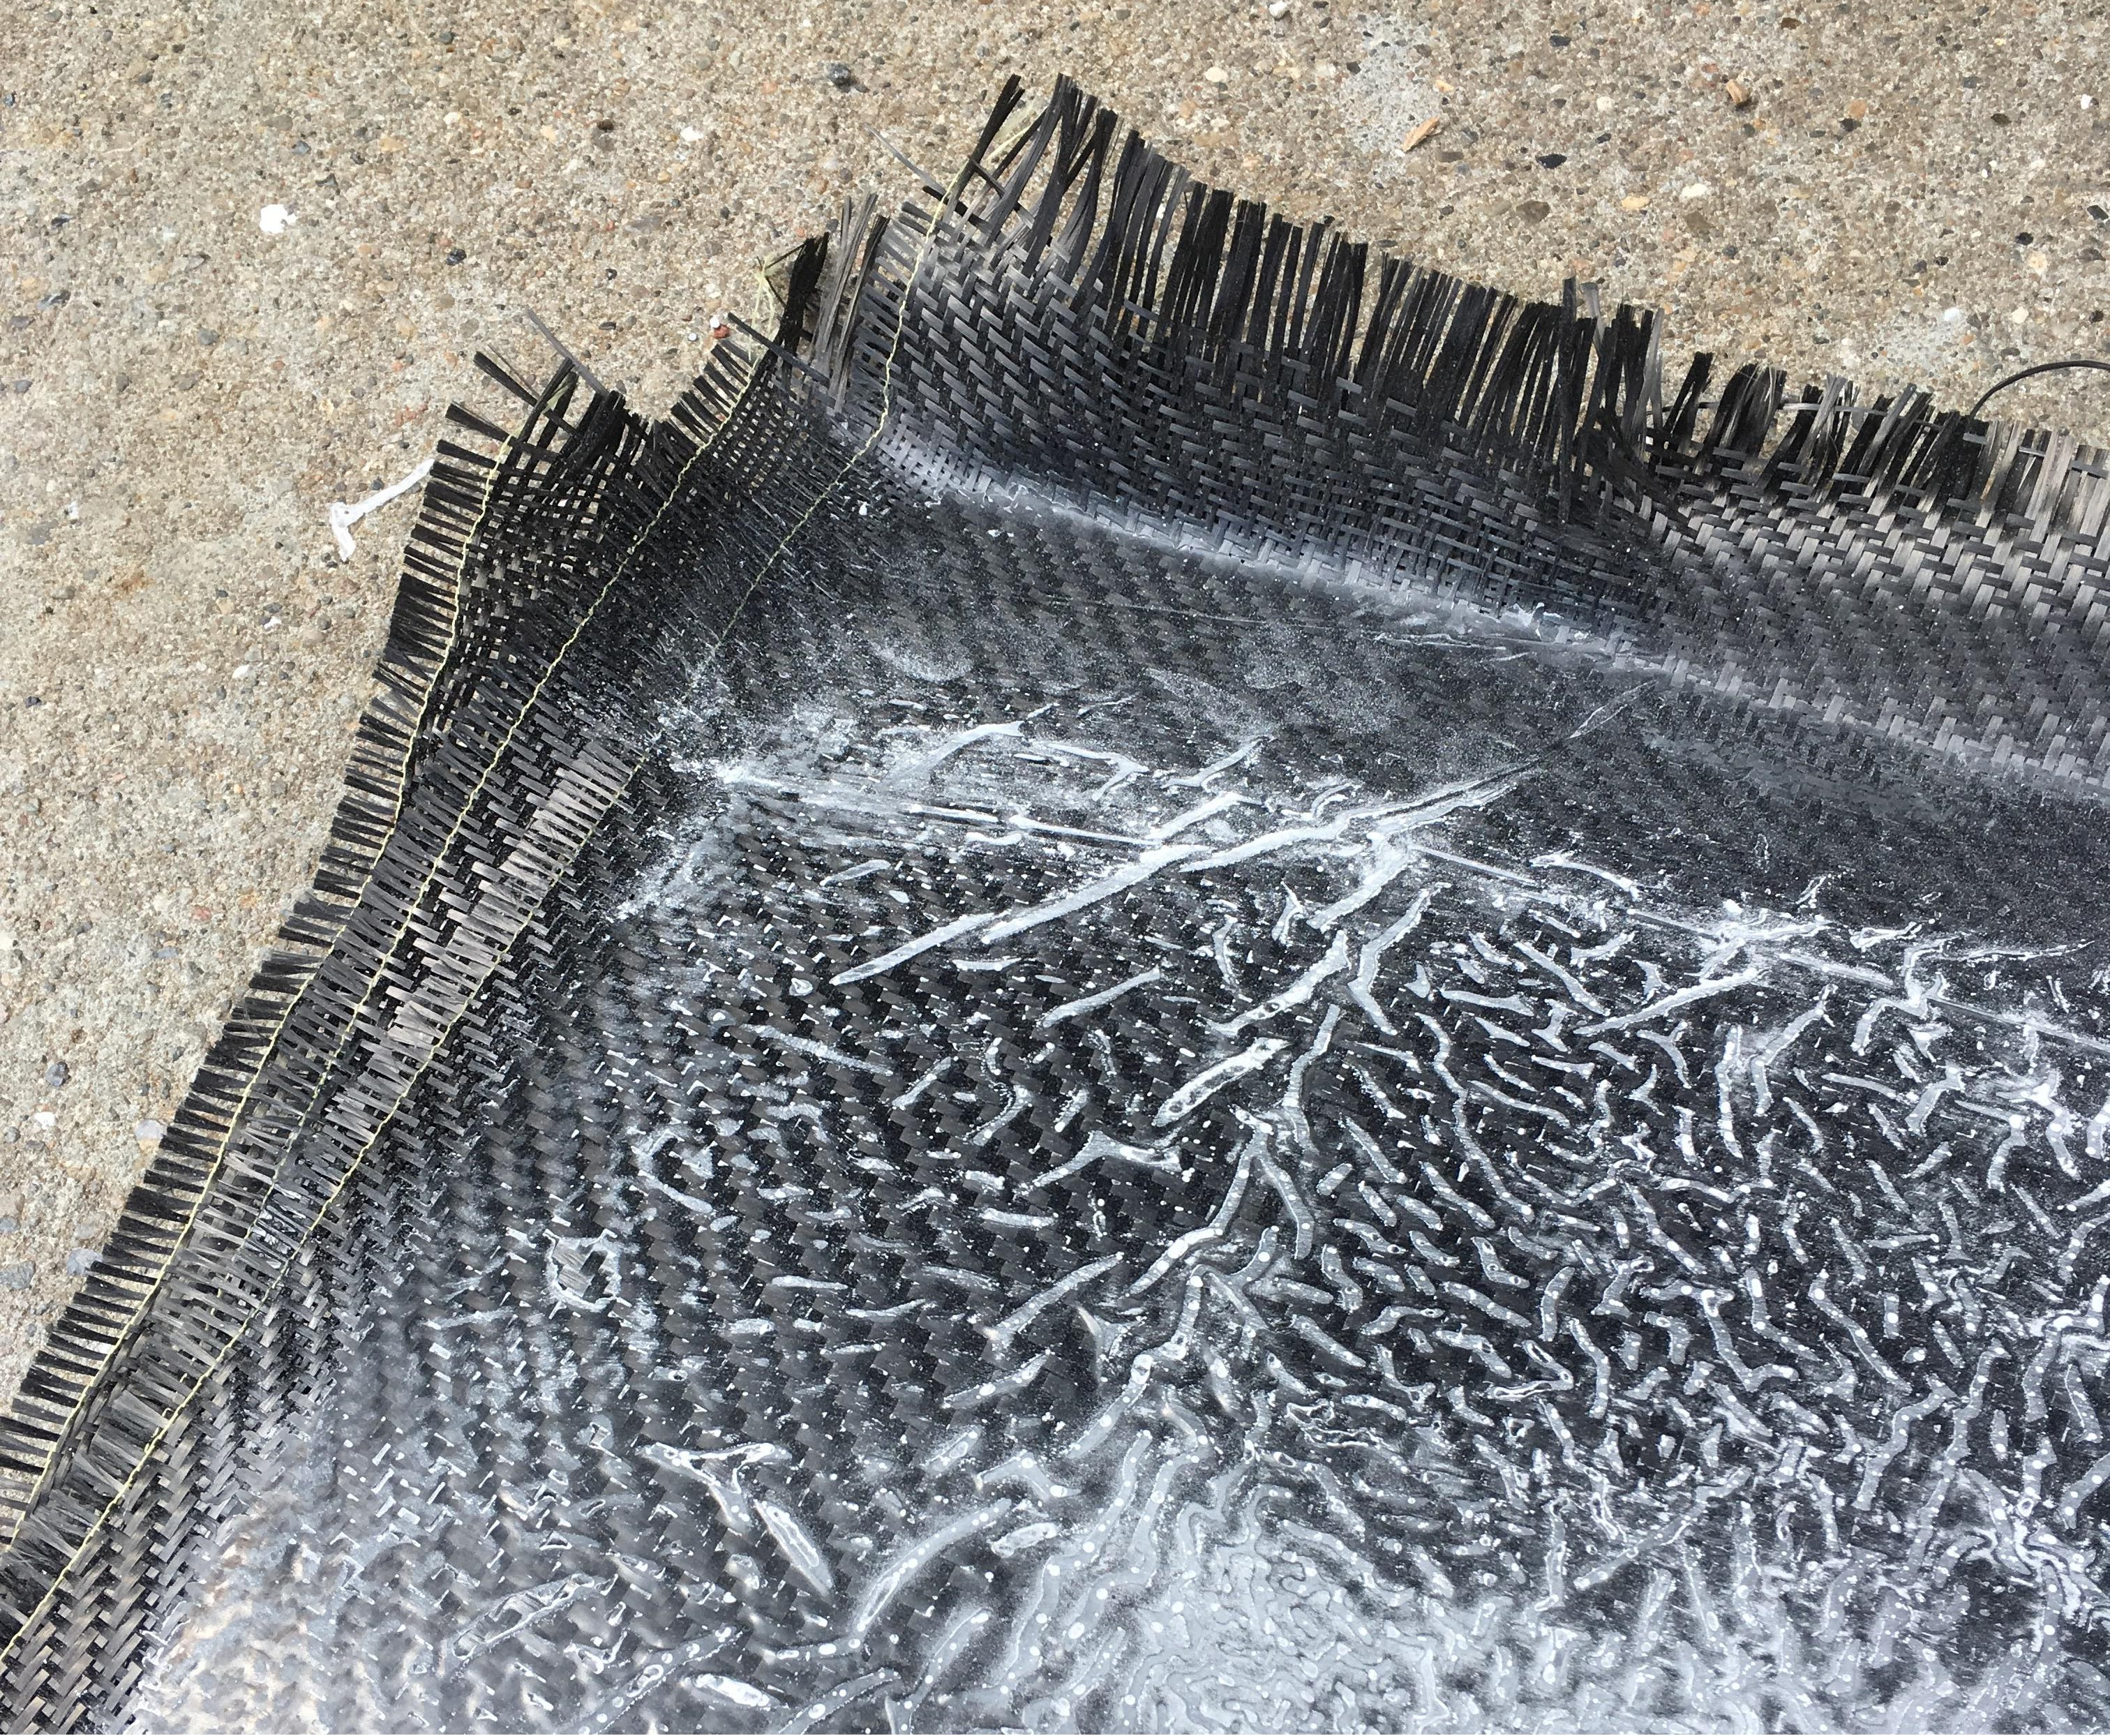
\includegraphics[width=\textwidth]{residualepoxy}
      \caption{Curing the wing in a flat position let the resin pool in the center of the wing, making the surface very rough.}
      \label{fig:roughsurface}
    \end{figure}

    \begin{figure}
      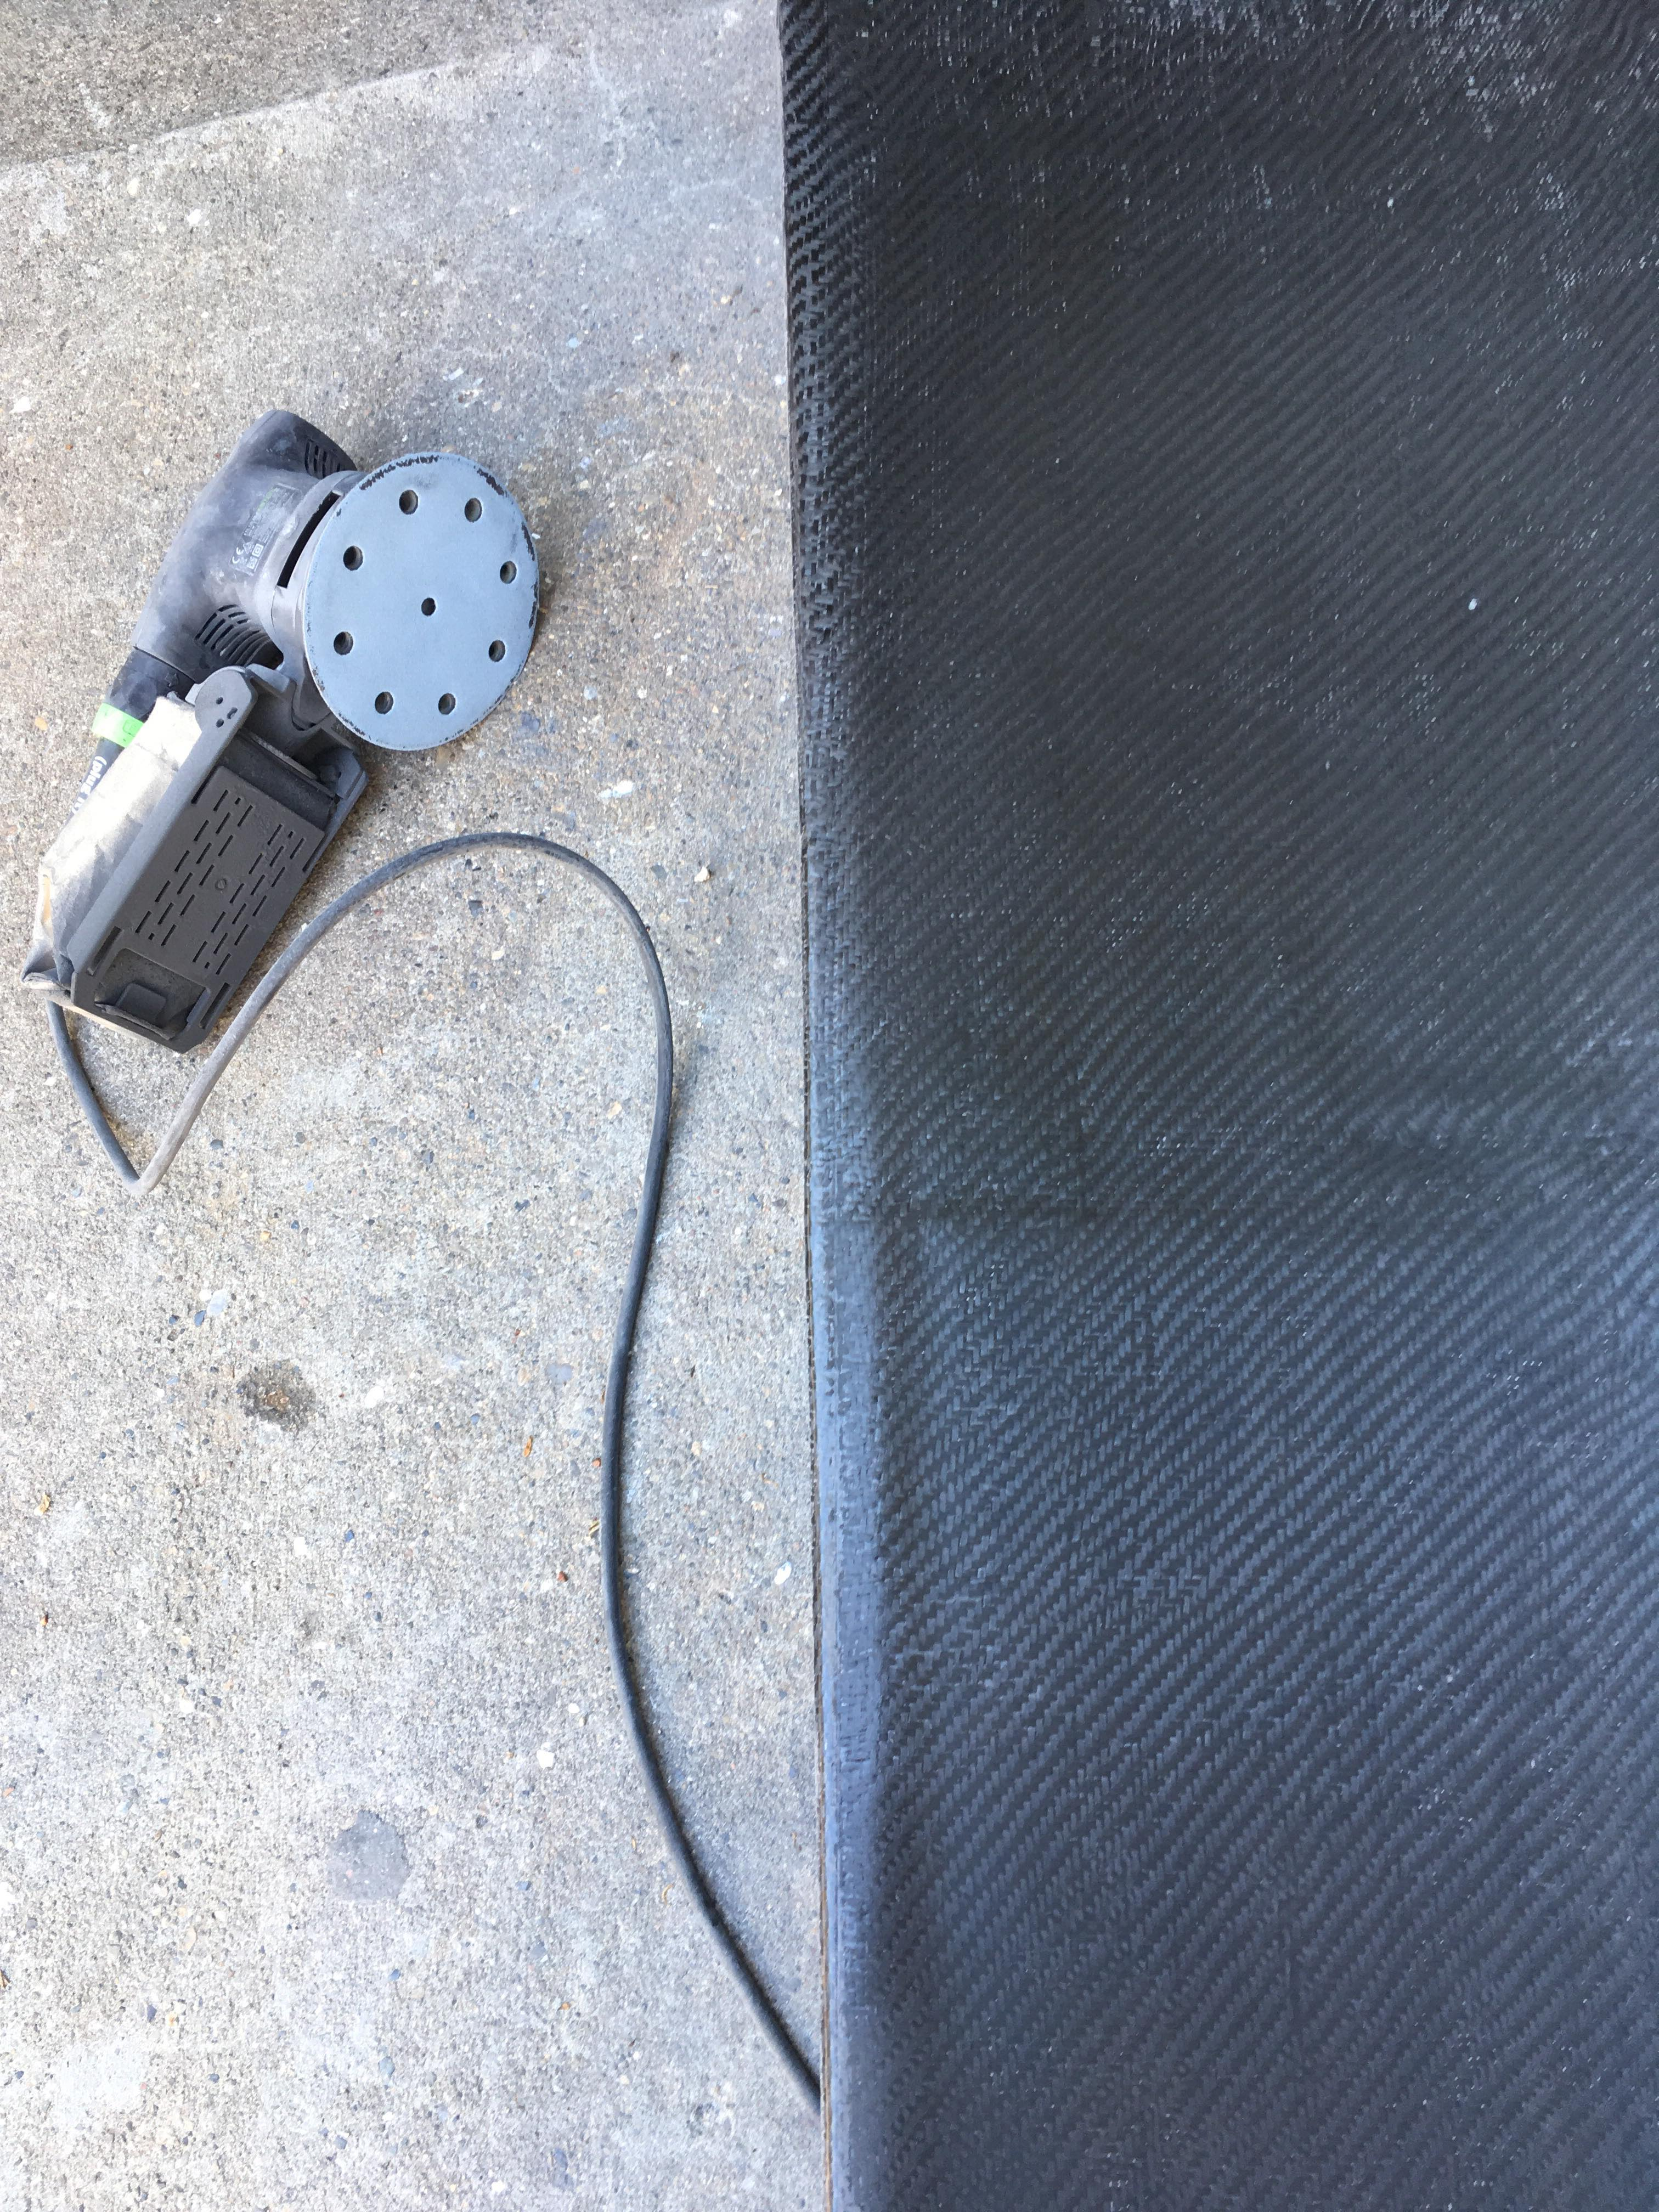
\includegraphics[width=\textwidth]{wingaftersanding}
      \caption{Sanding the wing clears the surface roughness, but requires a new layer of sealant. Using epoxy or a lacquer was investigated before settling on epoxy.}
      \label{fig:wingaftersanding}
    \end{figure}

  \subsection{Implementation and Testing}

\section{Testing and Inspection}

  \subsection{Reinforcing the mounting}
